\section{introduction}
In the era of information explosion, recommender systems have been playing a pivotal role in various online services~\cite{sarwar2001item}. Classic recommendation methods, e.g., matrix factorization~\cite{rendle2009bpr}, mainly model users' preference towards items using historical user-item interaction records. Nowadays, various kinds of auxiliary data become available in recommender systems, which can be leveraged to improve recommendation performance.
%Therefore, many methods leverage these context information to alleviate the cold-start problem, which widely exists in classic recommendation methods. 
%Due to the heterogeneity and complexity of auxiliary data, it is still challenging to model these information in recommender systems.
%Many methods further propose to leverage these context information for improving recommendation performance.
%Due to the heterogeneity and complexity of auxiliary data, it is still challenging to effectively utilize such context information in recommender systems. Besides, traditional recommendation methods focus on the interaction of single user and item while ignore the local information (\ie neighborhood information) of users and items.
%In the era of information explosion, recommender systems have playing an increasing important role in various online services, which aim to matcj
\begin{figure}
  \centering
  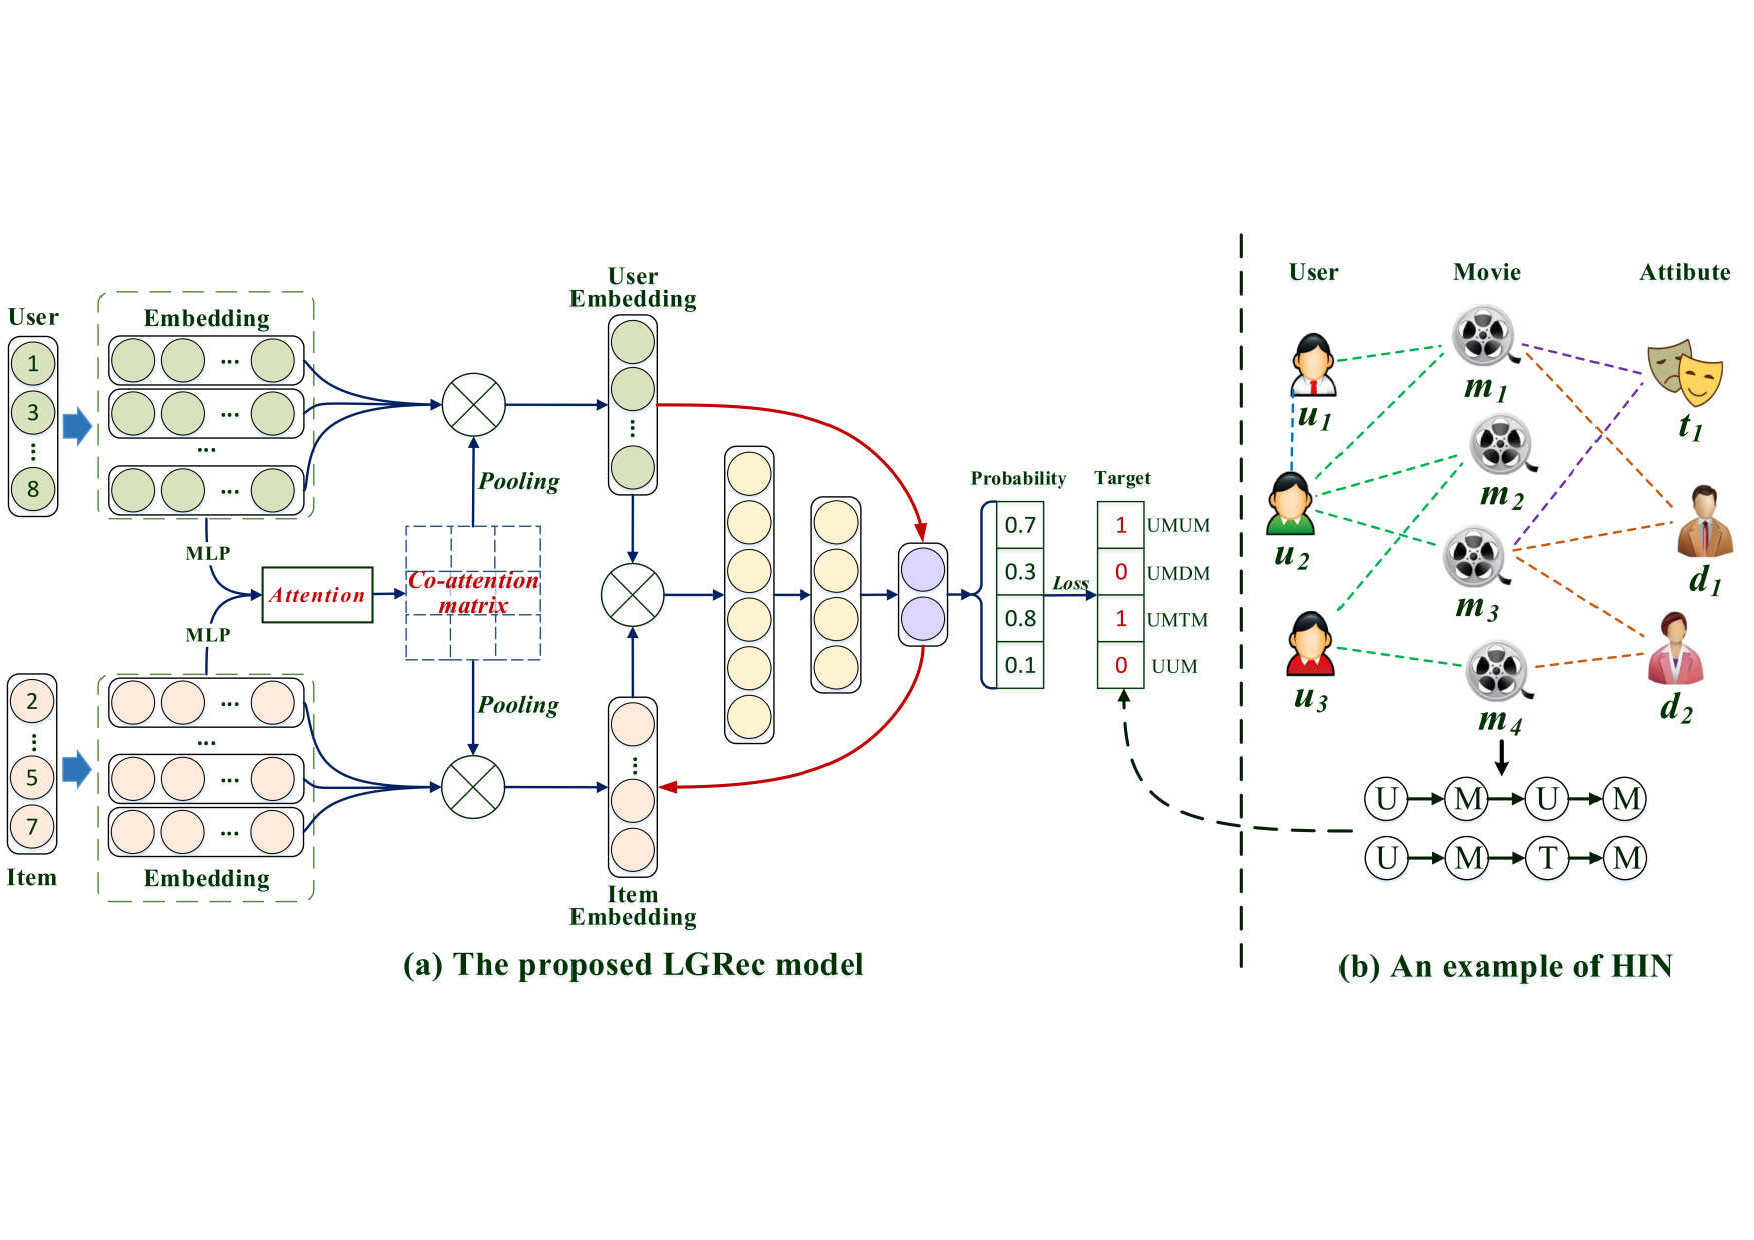
\includegraphics[width=8.5cm]{image/model.pdf}\\
  \caption{The overall architecture of the proposed model.}\label{fig-model}
\end{figure}

Recently, heterogeneous information network (HIN) , consisting of either multiple types of nodes or links, has been proposed as a powerful modeling method to fuse complex information, and is successfully applied to many data mining tasks~\cite{shi2017survey}. Moreover, meta-path~\cite{shi2017survey}, a relation sequence connecting objects, is widely used to effectively explore rich information and network structure in HIN.  Due to its flexibility in modeling data heterogeneity, HIN has also been adopted in recommender systems to characterize rich auxiliary data in recent years, and those algorithms are also called HIN based recommendation methods. In Fig.~\ref{fig-model}(b), we present an example for movie recommendation characterized by HIN. We can see that the HIN contains multiple types of entities connected by different types of relations. %And the meta-path $User-User$ (UU) indicates friendship between two users, while the meta-path $User-Movie-User$ (UMU) indicates the co-watch relation between users. 
And the meta-path $User-Movie-User-Movie$ (UMUM) indicates the historical interaction records between users and movies, while $User-Movie-Type-Movie$ (UMTM) indicates users prefer movies with the same type. Based on HIN, we further explore useful information for recommendation, namely \emph{local information} and \emph{global information}. Concretely, local information is direct interactions of users and items in HIN, while global information is indirect interactions between users and items based on different meta-paths. As we can see in Fig.~\ref{fig-model}(b), $u_3$ directly interacts with $m_2$ and $m_4$, which can be considered as the local information of $u_3$. Besides, $u_3$ can interact with $m_3$ through path $u_3 - m_2 - u_2 - m_3$ (UMUM) or path $u_3 - m_4 - d_2 - m_3$ (UMDM), which are the global information.     
%Recently, HIN has been adopted in recommender systems for characterizing complex and heterogenous recommendation settings, which can be called HIN based recommendation. 
%Some efforts~\cite{shi2017heterogeneous,zhao2017meta} have been made for HIN based recommendation, while they usually focus on rating prediction.



Existing HIN based recommendation methods~\cite{shi2017heterogeneous,zhao2017meta} usually leverage path based semantic relatedness of user-item pairs to enhance the representations of users and items for recommendation. 
%In addition, deep neural network is also been applied to learn the representations of users and items~\cite{he2017neural}.

Although these HIN based methods have achieved performance improvement to some extent, there are two shortcomings: 
(1) These methods tend to treat different local information equally, which is not an effective way to characterize these information for recommendation.
(2) They seldom exploit and explore local information and global information simultaneously. In HIN, besides the direct interactions (local information) between users and items, there widely exist meta-path based interactions (global information), which can potentially be integrated for recommendation.
%(1) These methods seldom extensively exploit local information. Although some network embedding based methods~\cite{shi2017heterogeneous} utilize local neighbor information with meta-paths, the embeddings of users and items are learned independently. 
%consider the local information (\ie direct interaction information), which is potential to construct more meaningful embedding for users and items. 
%(2) They seldom fully explore and exploit the global information (\ie meta-path based interaction information) in HINs for recommendation and most of previous works are proposed to model two-way interaction for recommender systems. 
%(2) They fail to fully explore the global information. In HIN, the different interactions between users and items can be modeled with meta-paths. Existing HIN based recommendation methods usually employ one meta-path or several assigned paths.
Based on these considerations, we aim to propose an unified model to extensively exploit the local interaction information and fully explore the global interaction information for top-$N$ recommendation. 
%To fulfill this purpose, we have to face two challenging issues: (1) Local information model (How to select the most informative local information to construct meaningful embedding); (2) Global information model (How to learn the relation embeddings for user-item pairs to uncover the rich heterogeneous information).

In order to comprehensively utilize local information, we assume that the embedding of a user (item) is determined by its connected items (users). Since different items (users) may have different contributions to the users (items), a co-attention mechanism is designed to automatically determine their weights. And then we explore and exploit rich information and network structure in HIN which is the global information can be modeled as the relation of each user-item pair. The learned representations can be regard as the composite interactions between users and items based on multiple meta-paths. Therefore a multi-label classification task is modeled to match the relation embdedding and interaction distribution on meta-paths.
%For the first issue, we consider that the embeddings of users (items) are influenced by their connected items (users). Hence,  we utilize a heuristic method to leverage useful local information (\ie neighborhood) and apply a co-attention mechanism to decide the importance of neighbors for constructing more meaningful embeddings for users and items. And then we learn the relation representation through the interaction between users and items based on MLP. On the other hand, each user-item pair can be connected by multiple meta-paths in HIN. After that, we match the relation representation and the distribution on meta-paths, which can be naturally formulated as multi-label classification problem. In this way, the learned relation representation can explore and exploit the rich information and network structure in HIN.
%we model the global information as multi-label classification problem to uncover rich information and network structure in HIN.
%And then we explore the rich information and network structure in HIN by capturing multiple meta-paths between user-item pairs and use them as prediction objectives simultaneously and jointly for learning of the relation representation.
Furthermore, we design a joint optimization objective to model the translation mechanism among users', items' representation and corresponding relation representation as well as the multi-label classification task for top-$N$ recommendation.
Extensive experiments on four real-world datasets demonstrate the effectiveness of the proposed model compared to the state of arts.
